\chapter{Synthesis in Example of a Magnetic Bearing on an Overhung Rotor}
Analysis and modeling techniques of the previous chapters will now be put to use in a practical example. The goal of which will be to balance an overhung disk rotor system with an Active Magnetic Bearing(AMB). An experimental test rig, not unlike the system used in the experimental example of /S\ref{ExperimentalPlots}, will be used to calibrate a  finite element theoretical model. Then, the theoretical model will be extended to include an AMB near the overhung disk. The model will be evaluated for stability, and parameters of the control algorithm for the AMB will be varied to attempt to eliminate the first natural frequency and stabilize the system.
\section{Physical System}

\section{Experimental Results}

\begin{figure}
	\centering
	\includegraphics[width=\linewidth]{./figures/MagExampleOrbit3D.pdf}
	\caption{3D Orbit of the experimental overhung rotor system.}
	\label{fig:MagExampleOrbit3D}
\end{figure}
\begin{figure}
	\centering
	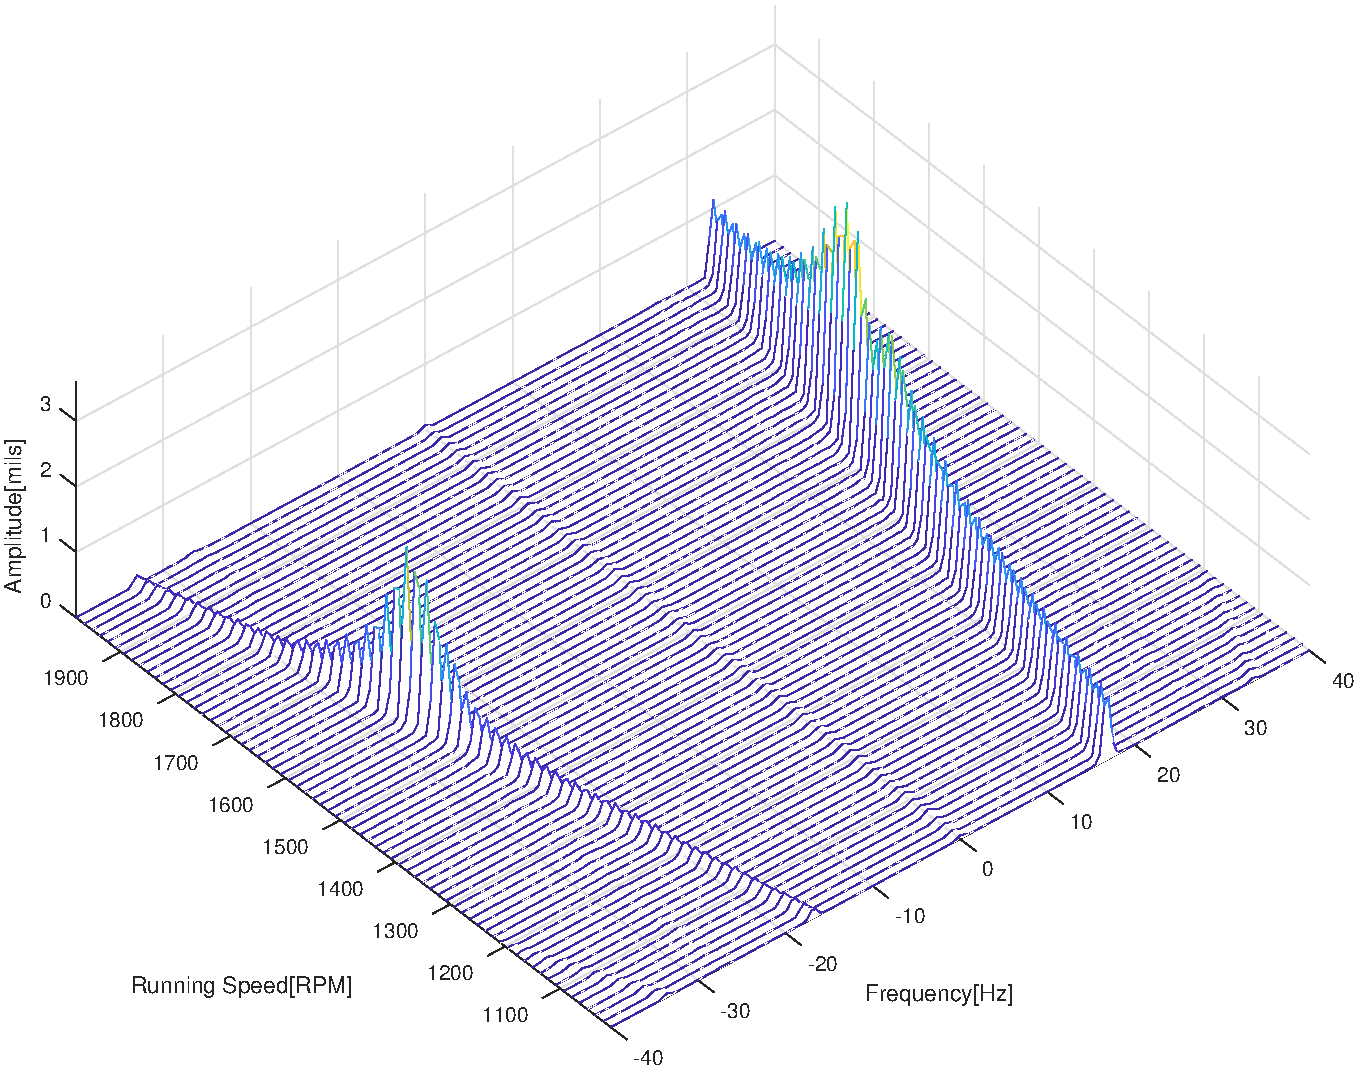
\includegraphics[width=\linewidth]{./figures/MagExampleCascade.pdf}
	\caption{Cascade of the experimental overhung rotor system.}
	\label{fig:MagExampleCascade}
\end{figure}
\begin{figure}[!htb]
	\def\width{.8\linewidth}
	\def\height{.4\linewidth}
	\def\sep{3em}
	\pgfplotsset{every picture/.style={trim axis left, trim axis right}, every axis/.style={ylabel style={xshift=0},xlabel style={yshift=0}}}%, every axis/.style={hide axis}}%
	\centering
	\import{figures/}{MagExampleBode.tex}
	\caption{Damping ratio vs. spin speed with indication of threshold of stability.}
	\label{fig:MagExampleBode}
\end{figure}
\section{Theoretical Model}
To create a theoretical model for this rotor system. The shaft will be discretized into 7 elements a disk at node 6 and bearings at nodes 1 and 4. In the experiment, a small length of shaft continued after the overhung disk and has been included in this model. The AMB will be included as a nodal point element with with stiffness and damping to be derived in \S\ref{Active Magnetic Bearing}.\par 
First the model is formed to match the experimental results. Known parameters, such as beam lengths, beam diameters, density of the material, and geometry of the disk are used to begin construction of the model. Then the campbell diagram is used to guess and check the stiffness for the bearings by comparing the first natural frequency of the model. After this process, the stiffness is determined to be around $ 2\e{5} \left[\frac{N}{m}\right]$. The diagram with this value of stiffness of all bearings in all directions is given as Figure \ref{fig:MagTheoryTuneCampbell}.
\begin{figure}[!htb]
	\def\width{.6\linewidth}
	\def\height{.4\linewidth}
	\def\sep{3em}
	\pgfplotsset{every picture/.style={trim axis left, trim axis right}, every axis/.style={ylabel style={yshift=.5em},xlabel style={yshift=0}}}%, every axis/.style={hide axis}}%
	\centering
	\import{figures/}{MagTheoryTuneCampbell.tex}
	\caption{Damping ratio vs. spin speed with indication of threshold of stability.}
	\label{fig:MagTheoryTuneCampbell}
\end{figure}
It is evident by inspection of the Bode diagram for the experimental system, fig.\ref{fig:MagExampleBode}, that there is anisotropy in the system, leading to the dip in amplitude of one plane of vibration. It is also known from inspection of the frequency spectrum in the cascade of figure \ref{fig:MagExampleCascade} that in this speed range the orbit is in the opposite direction of the rotation--a phenomena only possible with anisotropy of the stiffness. Figures \ref{fig:HorVertStiffAniCompare}\&\ref{fig:PosNegStiffAniCompare} demonstrate the effect anisotropy has on both the real coordinates, as well as positive and negative whirl amplitudes.\par 
\begin{figure}
	\centering
	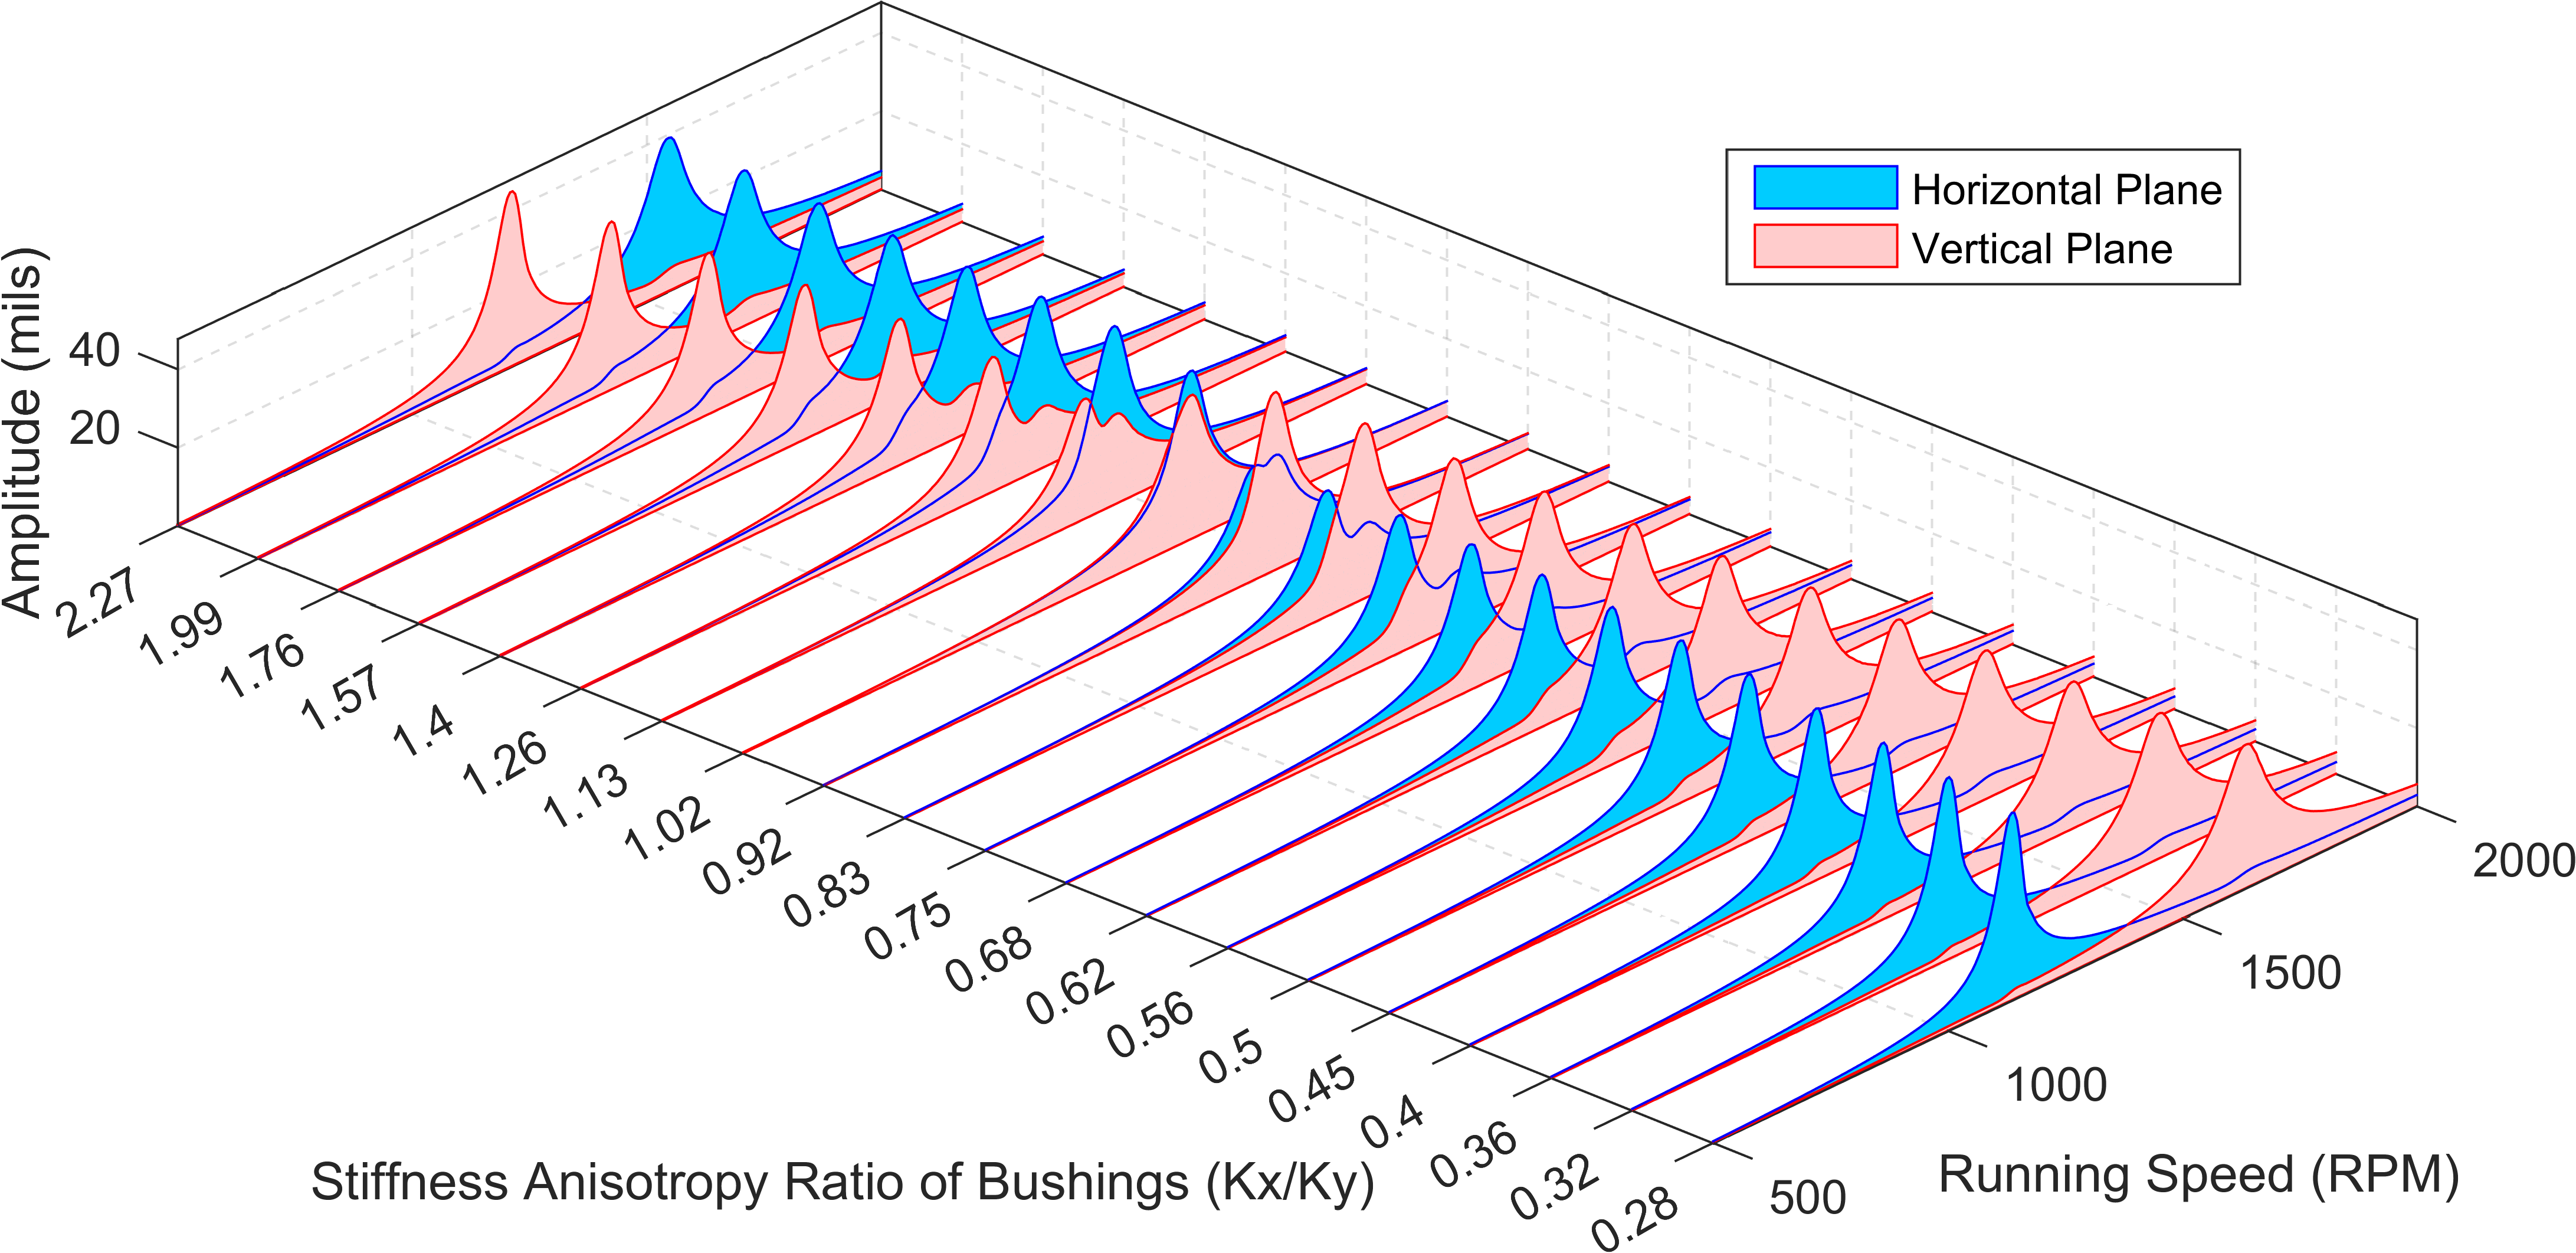
\includegraphics[width=\linewidth]{./figures/Images/Figure_6.png}
	\caption{3D Orbit of the experimental overhung rotor system.}
	\label{fig:HorVertStiffAniCompare}
\end{figure}
\begin{figure}
	\centering
	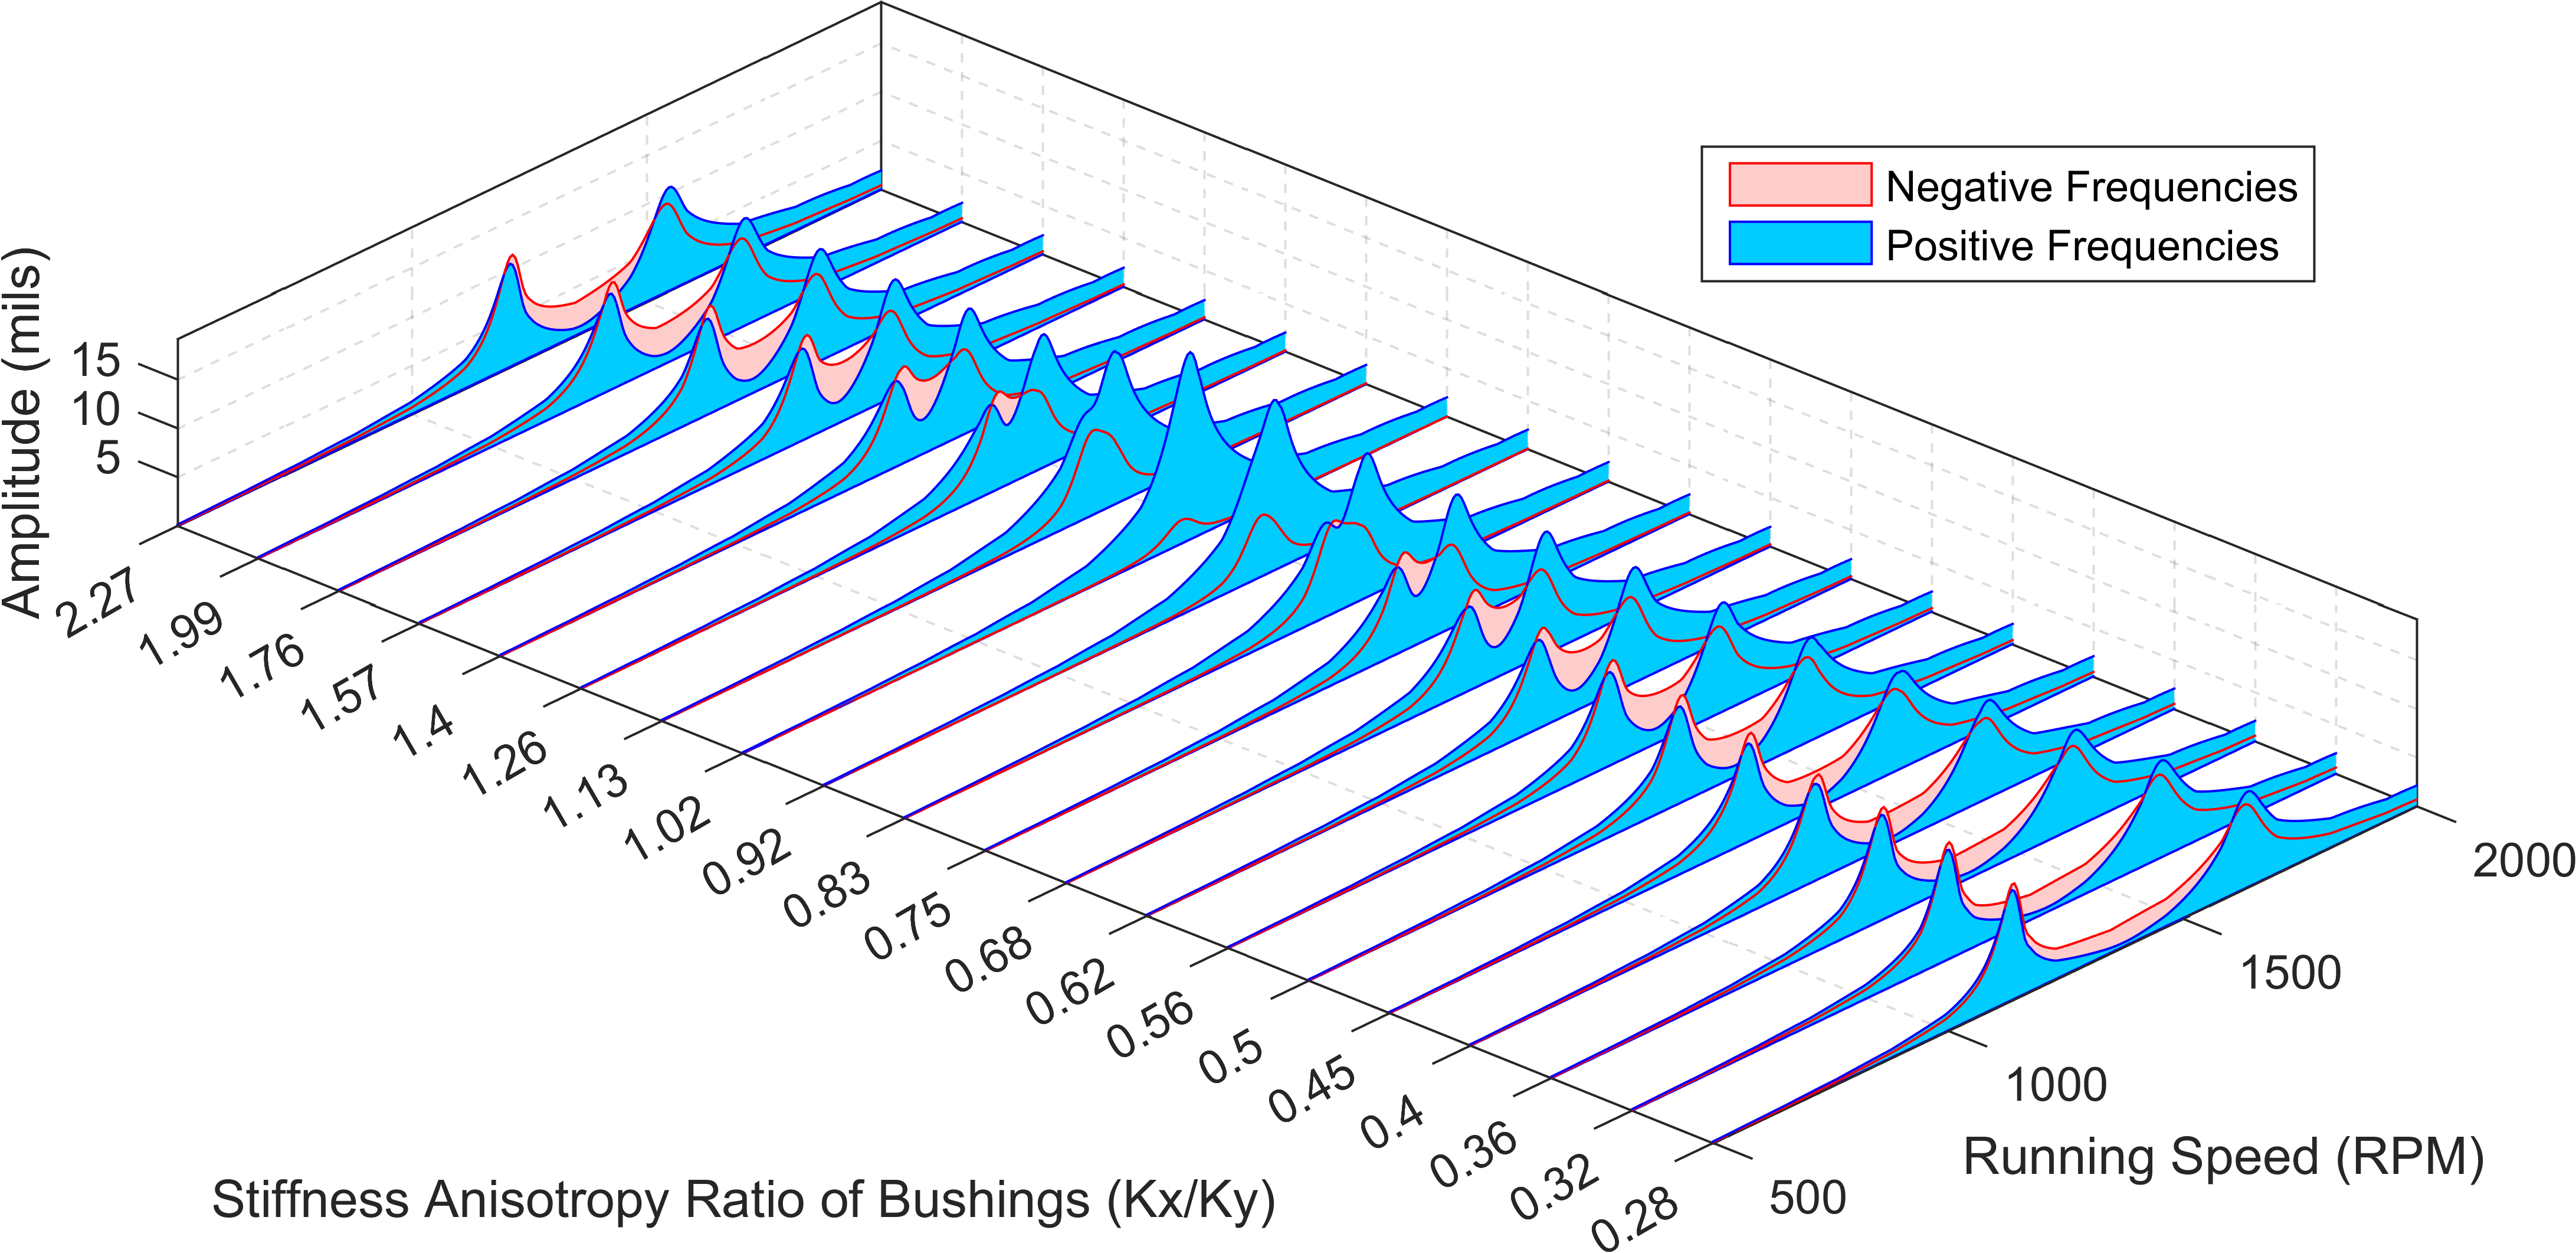
\includegraphics[width=\linewidth]{./figures/Images/Figure_5.png}
	\caption{3D Orbit of the experimental overhung rotor system.}
	\label{fig:PosNegStiffAniCompare}
\end{figure}
Using the bode diagram, the stiffness anisotropy is adjusted until the shapes of the amplitudes and phases match the experimental results of figure \ref{fig:ExpExampleBode}. Then damping is added to the system to appropriately match the experimental results. The resulting bode diagram is Figure \ref{fig:MagTheoryBode}. Stiffnesses were determined to be $ k_x=1.1\e{5}[N/m]\ \&\ k_y=1.5\e{5}[N/m] $.
\begin{figure}[!htb]
	\def\width{.6\linewidth}
	\def\height{.4\linewidth}
	\def\sep{3em}
	\pgfplotsset{every picture/.style={trim axis left, trim axis right}, every axis/.style={ylabel style={yshift=.5em},xlabel style={yshift=0}}}%, every axis/.style={hide axis}}%
	\centering
	\import{figures/}{MagTheoryBode.tex}
	\caption{Damping ratio vs. spin speed with indication of threshold of stability.}
	\label{fig:MagTheoryBode}
\end{figure}
And now the resulting system is further described with the new Campbell diagram in Figure \ref{fig:MagTheoryCampbell}, the roots locus in Figure \ref{fig:MagTheoryRootLocus}
\begin{figure}[!htb]
	\def\width{.6\linewidth}
	\def\height{.4\linewidth}
	\def\sep{3em}
	\pgfplotsset{every picture/.style={trim axis left, trim axis right}, every axis/.style={ylabel style={yshift=.5em},xlabel style={yshift=0}}}%, every axis/.style={hide axis}}%
	\centering
	\import{figures/}{MagTheoryCampbell.tex}
	\caption{Damping ratio vs. spin speed with indication of threshold of stability.}
	\label{fig:MagTheoryCampbell}
\end{figure}
\begin{figure}[!htb]
	\def\width{.6\linewidth}
	\def\height{.4\linewidth}
	\def\sep{3em}
	\pgfplotsset{every picture/.style={trim axis left, trim axis right}, every axis/.style={ylabel style={yshift=.5em},xlabel style={yshift=0}}}%, every axis/.style={hide axis}}%
	\centering
	\import{figures/}{MagTheoryRootLocus.tex}
	\caption{Damping ratio vs. spin speed with indication of threshold of stability.}
	\label{fig:MagTheoryRootLocus}
\end{figure}
\begin{figure}
	\def\cs{.29}
	\begin{subfigure}{\cs\textwidth}
		\centering
		\def\width{\linewidth+.8em}
		\def\height{\linewidth}
		\def\sep{3em}
		\pgfplotsset{every picture/.style={trim axis left, trim axis right}, every axis/.style={yticklabel style={xshift=.4em,yshift=.4em},minor tick num=2}, grid style={line width=.1pt, draw=gray!10},major grid style={line width=.2pt,draw=gray!50},}%, every axis/.style={hide axis}}%
		\import{figures/}{MagTheoryShape1.tex}
		\caption{Mode Shape 1.}
		\label{fig:MagTheoryShape1}
	\end{subfigure}
	\begin{subfigure}{\cs\textwidth}
		\centering
		\def\width{\linewidth+1em}
		\def\height{\linewidth}
		\def\sep{3em}
		\pgfplotsset{every picture/.style={trim axis left, trim axis right}, every axis/.style={yticklabel style={xshift=.4em,yshift=.4em},minor tick num=2}, grid style={line width=.1pt, draw=gray!10},major grid style={line width=.2pt,draw=gray!50},}%, every axis/.style={hide axis}}%
		\import{figures/}{MagTheoryShape2.tex}
		\caption{Mode Shape 2.}
		\label{fig:MagTheoryShape2}
	\end{subfigure}
	\begin{subfigure}{\cs\textwidth}
		\centering
		\def\width{\linewidth+1em}
		\def\height{\linewidth}
		\def\sep{3em}
		\pgfplotsset{every picture/.style={trim axis left, trim axis right}, every axis/.style={yticklabel style={xshift=.4em,yshift=.4em},minor tick num=2}, grid style={line width=.1pt, draw=gray!10},major grid style={line width=.2pt,draw=gray!50},}%, every axis/.style={hide axis}}%
		\import{figures/}{MagTheoryShape3.tex}
		\caption{Mode Shape 3.}
		\label{fig:MagTheoryShape3}
	\end{subfigure}
\end{figure}
\subsection{Active Magnetic Bearing}\label{Active Magnetic Bearing}
A single radial pair magnetic pole-rotor relationship will be derived based on the detailed derivation in \cite{das2008vibration}. Assumptions made in this model are:
\begin{itemize}
	\item Air gap between the magnet pole face and the rotor is vanishingly small compared to the diameter of the shaft.\
	\item Flux leakage from the magnetic pole is negligible.
	\item Curvature of rotor surface under the pole face is ignored.
	\item A linear relationship of flux density and magnetic field is assumed.
	\item Hysteresis of the magnetic field is negligible.
\end{itemize}
These assumptions lead to a magnetic force due to coil current in the relationship of
\begin{equation}\label{key}
F_m=\frac{-k_mi^2}{l_g^2}
\end{equation}
where, $ k_m=\frac{\mu_0A_pN^2}{4} $, and $ \mu_0=4\pi\e{-7} $ is the absolute permeability in free air, $ N $ is the number of coil turns, $ A_p $ is the pole face area, $ i $ is the supplied electrical current, and $ l_g $ is the air gap.\par 
Consider a sets of magnetic poles in the $ y\ \&\ z $ directions (i.e. One pair on the left and one pair on the right), where each pair of poles has its own electrical circuit. All sets of poles in the neutral position of the system will have a nominal air gap of $ g_0 $ and will be supplied by a bias current of $ i_0 $. Deviations of the current from this bias will be considered as $ i_y $ and $ i_z $. Deviations of the position from this neutral position are the displacements of the rotor at this beam axis location, $ v,\ \&\ w $. Therefore, total current will be $ (i_0\pm i_y)\ \&\ (i_0\pm i_z) $ for opposing poles in the $ y\ \&\ z $ directions respectively. Similarly, total gaps are given by $ (g_0\pm v)\ \&\ (g_0\pm w) $. Using these new definitions for the gap and current, an summing forces in the $ y\ \&\ z $ directions leads to the total force
\begin{equation}\label{eq:MagneticForceNL}
F_y=K_m\left\{\left(\frac{i_0+i_y}{g_0+v}\right)^2-\left(\frac{i_0-i_y}{g_0-v}\right)^2\right\}\ \&\ F_z=K_m\left\{\left(\frac{i_0+i_z}{g_0+w}\right)^2-\left(\frac{i_0-i_z}{g_0-w}\right)^2\right\}
\end{equation}
where, $ K_m=k_m\cos(\alpha) $, and $ \alpha $ is half of the angle between the poles forming a pair. Linearizing the magnetic force equations \eqref{eq:MagneticForceNL}, while assuming the operating point for the system is where all positions and control currents are zero, results in
\begin{equation}\label{eq:MagneticForce}
F_y=k_ii_y+k_yv,\ \&\ F_z=k_ii_z+k_zw
\end{equation}
where, $ k_i=4K_m\frac{i_0}{g_0^2} $ is the current stiffness developed by the bias current, and $ k_y=k_z=k_s=-4K_m\frac{i_0^2}{g_0^3} $.
\subsubsection{Proportional Derivative Control}
A control algorithm is used to control the current sent to each pair of poles based on the position (proportional) and velocity (derivative) of the rotor. It is assumed that each set of pole pairs will receive opposite currents to act as a unit. Current control is given by 
\begin{equation}\label{eq:ControlCurrent}
i_y=-k_g(k_pv+k_v\dot{v}),\ \&\ i_z=-k_g(k_pw+k_v\dot{w})
\end{equation}
where, $ k_g $ is the power amplifier gain, $ k_p $ is the proportional gain, and $ k_v $ is the derivative gain. The total linearized force becomes
\begin{equation}\label{key}
F_y=-(k_gk_ik_p-k_s)v-k_gk_ik_v\dot{v},\ \&\ F_z=-(k_gk_ik_p-k_s)w-k_gk_ik_v\dot{w}
\end{equation}
so then the stiffness of the AMB is $ k_{mag}=(k_gk_ik_p-k_s) $ and the damping is $ d_{mag}=k_gk_ik_v $. As an equation of nodal stiffness and damping in the finite element system it can be represented by
\begin{equation}\label{eq:DiskNodeEquationofMotion}
\bunderline{\mathbf{D}}^m\dot{\vec{\mathbf{q}}}_k+\bunderline{\mathbf{K}}^m\vec{\mathbf{q}}_k=0
\end{equation}
where,
\begin{equation*}
\def\cs{2em}
\begin{array}{cc}
\bunderline{\mathbf{K}}^m=\left[\def\arraystretch{.8}\arraycolsep=0pt\begin{array}{cccccc}
\makebox[\cs]{$k_{mag}$}&\makebox[\cs]{0}&\makebox[\cs]{0}&\makebox[\cs]{0}&\makebox[\cs]{0}&\makebox[\cs]{0}\\
0&k_{mag}&0&0&0&0\\
0&0&0&0&0&0\\
0&0&0&0&0&0\\
0&0&0&0&0&0\\
0&0&0&0&0&0
\end{array}\right] & \bunderline{\mathbf{D}}^m=\left[\def\arraystretch{.8}\arraycolsep=0pt\begin{array}{cccccc}
\makebox[\cs]{$d_{mag}$}&\makebox[\cs]{0}&\makebox[\cs]{0}&\makebox[\cs]{0}&\makebox[\cs]{0}&\makebox[\cs]{0}\\
0&d_{mag}&0&0&0&0\\
0&0&0&0&0&0\\
0&0&0&0&0&0\\
0&0&0&0&0&0\\
0&0&0&0&0&0
\end{array}\right]
\end{array}
\end{equation*}
\section{Addition of Magnetic Bearing}
In order to measure the effectiveness of the AMB, the Stability of the theoretical model before the addition is shown in Figure \ref{fig:MagTheoryStability}. The magnetic bearing added is modeled after a magnetic bearing that is currently in the lab at California Polytechnic State University. This theoretical exercise is intended to be followed by experimental verification, not included in this work. The parameters used are listed in \ref{tab:MagBearingParameters}. To determine best derivative control, the proportional control was set to zero and the derivative increased until the first mode on the Roots locus(fig. \ref{fig:MagTheoryRootLocus}) moved away from the real axis. Then proportional was added. The resulting movement of the Roots on the Roots Locus is given in Figure \ref{fig:MagTheoryRootsLocusWith}. Notice haw none of the new modes that appear on the roots locus cross the real plane--this demonstrates the stability of the new system. Stability of the system with the AMB addition is confirmed in the stability plot of Figure \ref{fig:MagTheoryStabilityWith}
\begin{table}
	\centering\label{tab:MagBearingParameters}
	\caption{Active Magnetic Bearing Parameters.}
	\begin{tabular}{cccccccc}
		$\alpha[rad]$&$g_0[m]$&$i_0[A]$&$k_p[\frac{V}{m}]$&$k_v[\frac{Vs}{m}]$&$k_g[\frac{A}{V}]$&$ N[\#]$&$A_p[m^2]$\\\hline
		$\frac{\pi}{8}$&$2.5\e{-3}$&$5$&$2000$&$20$&$0.8$&$800$&$\frac{5}{100*100}$
		\end{tabular}
\end{table}
\begin{figure}[!htb]
	\def\width{.6\linewidth}
	\def\height{.4\linewidth}
	\def\sep{3em}
	\pgfplotsset{every picture/.style={trim axis left, trim axis right}, every axis/.style={ylabel style={yshift=-.5em},xlabel style={yshift=5em}}}%, every axis/.style={hide axis}}%
	\centering
	\import{figures/}{MagTheoryStability.tex}
	\caption{Damping ratio vs. spin speed with indication of threshold of stability.}
	\label{fig:MagTheoryStability}
\end{figure}
\begin{figure}[!htb]
	\def\width{.6\linewidth}
	\def\height{.4\linewidth}
	\def\sep{3em}
	\pgfplotsset{every picture/.style={trim axis left, trim axis right}, every axis/.style={ylabel style={yshift=-30em},xlabel style={yshift=0em}}}%, every axis/.style={hide axis}}%
	\centering
	\import{figures/}{MagTheoryRootsLocusWith.tex}
	\caption{Roots locus of Overhung rotor system without AMB(Black), and with AMB(Blue).}
	\label{fig:MagTheoryRootsLocusWith}
\end{figure}
\begin{figure}[!htb]
	\def\width{.6\linewidth}
	\def\height{.4\linewidth}
	\def\sep{3em}
	\pgfplotsset{every picture/.style={trim axis left, trim axis right}, every axis/.style={ylabel style={yshift=0em},xlabel style={yshift=19em}}}%, every axis/.style={hide axis}}%
	\centering
	\import{figures/}{MagTheoryStabilityWith.tex}
	\caption{Roots locus of Overhung rotor system without AMB(Black), and with AMB(Blue).}
	\label{fig:MagTheoryStabilityWith}
\end{figure}
\begin{figure}[!htb]
	\def\width{.6\linewidth}
	\def\height{.4\linewidth}
	\def\sep{3em}
	\pgfplotsset{every picture/.style={trim axis left, trim axis right}}%, every axis/.style={ylabel style={yshift=0em},xlabel style={yshift=0}}}%, every axis/.style={hide axis}}%
	\centering
	\import{figures/}{MagTheoryFreqResponseCompare.tex}
	\caption{Roots locus of Overhung rotor system without AMB(Black), and with AMB(Blue).}
	\label{fig:MagTheoryFreqResponseCompare}
\end{figure}
